\section{Listen}

\textbf{Sequenzen} sind \textbf{Folgen} bzw.\textbf{Listen}, auf denen eine Ordnung definiert ist (\textit{erstes Element}, \textit{zweites Element}, ... \textit{n-tes Element}).\\

\noindent
Bei einer Liste sind Elemente miteinander \textit{verkettet}: Die Größe einer Liste kann dadurch dynamisch wachsen und es muss nicht vorher die Größe der Liste zur Aufnahme von $n$ Elementen festgelegt werden (wie bei Feldern).\\

\noindent
Ein Element in einer Liste zeigt auf einen \textbf{Nachfolger} \code{succ} und je nach Implementierung auf einen \textbf{Vorgänger} \code{pred}.\\
Hat ein Element keinen Nachfolger oder Vorgänger, ist der jeweilige Zeiger der \textbf{Nullzeiger}\footnote{
s. a.~\cite[49 f.]{GD18b} sowie ``Nullzeiger``: \url{https://de.wikipedia.org/wiki/Zeiger_(Informatik)#Nullzeiger} - abgerufen 09.03.2024
}.

\subsection{Einfach verkettete Liste}
In einer \textbf{einfach verketteten Liste} zeigen Listenelemente nur auf ihren Nachfolger.\\

\noindent
Ein \textit{Dummy-Element} \code{head} zeigt auf das erste Listenelement bzw. auf \code{null}, falls die Liste leer ist.\\

\noindent
Alternativ zeigt ein \textit{Dummy-Elemente} \code{head} auf das erste und ein Dummy-Element \code{tail} auf das letzte Listenelement - hierdurch lassen sich Operationen wie \code{last()} und \code{concat()} effizienter implementieren (s. Abbildung~\ref{fig:linkedlist}).

\begin{figure}
    \begin{center}
        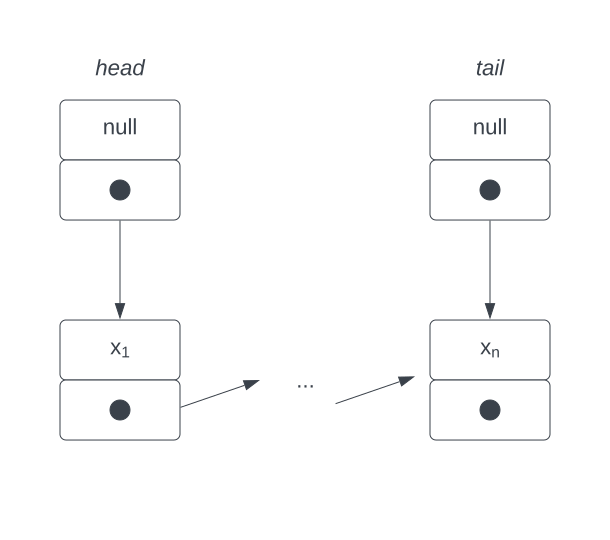
\includegraphics[scale=0.4]{chapters/Datenstrukturen und Algorithmen/img/linkedlist}
        \caption{Einfach verkettete Liste mit Zeigern auf das erste und das letzte Listenelement. (Quelle: eigene)}
        \label{fig:linkedlist}
    \end{center}
\end{figure}

\subsection{Doppelt verkettete Liste}
In einer \textbf{doppelt verketteten Liste} zeigen Listenelemente auf ihren Nachfolger \textit{und} ihren Vorgänger.\\

\noindent
Ein \textit{Dummy-Element} \code{head} zeigt mit \code{pred} auf das Ende der Liste und mit \code{succ} auf das erste Listenelement (s. Abbildung~\ref{fig:doublelinkedlist}).\\

\noindent
Doppelt verkettete Listen verbrauchen mehr Speicher, da sie mehr Zeiger verwenden ($2*m + 2$, $m = $ Anzahl der Listenelemente, $+2$ für die \code{head}- / \code{tail}-Zeiger).

\begin{figure}
    \begin{center}
        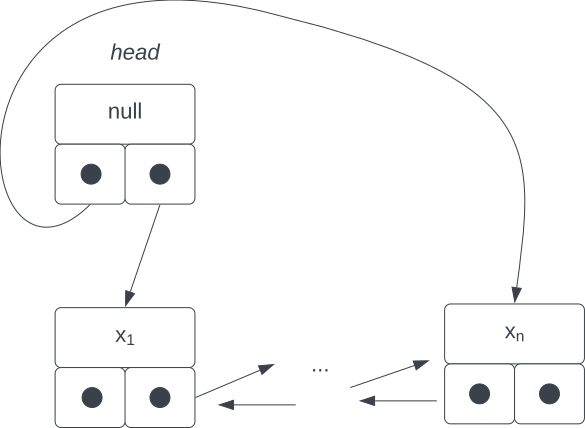
\includegraphics[scale=0.4]{chapters/Datenstrukturen und Algorithmen/img/doublelinkedlist}
        \caption{Doppelt verkettete Liste. Das Kopfelement zeigt auf das erste und das letzte Listenelement mit \textit{succ} bzw. \textit{pred}. (Quelle: eigene)}
        \label{fig:doublelinkedlist}
    \end{center}
\end{figure}

\subsection{Darstellung im Array}
Eine Liste kann auch in einem Array dargestellt werden.\\
Hierfür muss in Java jedoch entsprechend Speicherplatz für das Array reserviert werden - der je nach Anzahl der Einträge nicht ausgefüllt wird oder nicht ausreicht.\\
In letzteren Fall kann es dazu führen, dass neue Elemente nicht in das Array passen und deshalb ein neues Array angefordert werden muss.
In diesem Fall müssen alle Einträge in das neue Array kopiert werden.


\subsection{Laufzeiten}

Die Laufzeiten für die verschiedenen Listenimplementierungen sind in Tabelle~\ref{tab:listruntime} zusammengefasst.\\

\noindent
Die doppelt verkettete Liste ist bei den Operationen \textit{einfügen} und \textit{entfernen} im Vorteil, da Zeiger auf die Vorgängerelemente existieren.
Hierdurch muss nicht zunächst - wie in einer einfach verketteten Liste - das Vorgängerelement gesucht werden, dessen \code{succ}-Zeiger angepasst werden muss.\\
Die Laufzeiten in der Array-Implementierung sind dadurch bedingt, dass Folgeelemente geshifted werden müssen - wird bspw. das erste Element gelöscht, müssen n-1 Folgeelemente nach links verschoben werden.

\setlength{\tabcolsep}{1.5em}
\renewcommand{\arraystretch}{1.5}%
\begin{table} %[hbtp]
    \centering
    \begin{tabular}{|l | c | c | c|}
        \hline
                            & verkettete Liste & doppelt verkettete Liste & Liste als Array \\
        \hline
        \textit{suchen}     &    $O(n) $    &    $O(n)$      & $O(n)$ \\
        \hline
        \textit{einfügen}   &    $O(n) $    &    $O(1)$      & $O(n)$ \\
        \hline
        \textit{entfernen}  &    $O(n) $    &    $O(1)$     &  $O(n)$\\
        \hline
    \end{tabular}
    \caption{Laufzeiten für die Operationen \textit{suchen}, \textit{einfügen} und \textit{entfernen} bei verschiedenen Listenimplementierungen.}
    \label{tab:listruntime}
\end{table}